\documentclass[tikz, border=10pt]{standalone}
\usepackage{tikz}
\usetikzlibrary{calc}

\begin{document}
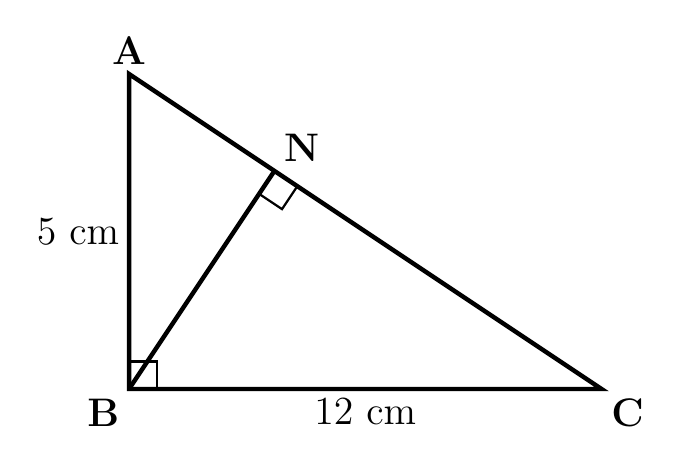
\begin{tikzpicture}

% Define vertices
\coordinate (B) at (0, 0);
\coordinate (A) at (0, 4);
\coordinate (C) at (6, 0);

% Calculate N (foot of altitude from B to AC)
\coordinate (N) at ($(A)!(B)!(C)$);

% Draw the triangle
\draw[ultra thick] (A) -- (B) -- (C) -- cycle;

% Draw altitude BN
\draw[ultra thick] (B) -- (N);

% Right angle mark at B (angle ABC)
\def\sq{0.35}
\draw[thick] (B) ++(0,\sq) -- ++(\sq,0) -- ++(0,-\sq);

% Right angle mark at N (using rotation)
\begin{scope}[shift={(N)}, rotate={-atan2(4,6)}]
    \draw[thick] (0,-\sq) -- ++(\sq,0) -- ++(0,\sq);
\end{scope}

% Labels for vertices
\node[above] at (A) {\textbf{\Large A}};
\node[below left] at (B) {\textbf{\Large B}};
\node[below right] at (C) {\textbf{\Large C}};
\node[above right] at (N) {\textbf{\Large N}};

% Left side: AB = 5 cm
\node[left, font=\Large] at ($(A)!0.5!(B)$) {5 cm};

% Bottom side: BC = 12 cm
\node[below, font=\Large] at ($(B)!0.5!(C)$) {12 cm};

\end{tikzpicture}
\end{document}